\newpage
\section{Fundamental Solutions to the Wave Equation}

\subsection{Lorentz invariance of fundamental solution}
Last time, we were solving the wave equation
where
$$
\begin{aligned}
\square &=\partial_{t}^{2}-\Delta_{x} \\
&=m^{\alpha, \beta} \partial_{\alpha} \partial_{\beta}
\end{aligned}
$$
in coordinates $t=x_{0}$ and $\partial_{t}=\partial_{0}$. The matrix $M$ is given by
$$
M=\left[\begin{array}{llll}
-1 & & & \\
& 1 & & \\
& & \ddots & \\
& & & 1
\end{array}\right]
$$
Last time, we determined that a fundamental solution is homogeneous of order $1-n$ and must move forward in time. We looked at symmetries of the equation when we make a linear change of coordinates $x=A y$. We saw that such a linear change of coordinates leaves $\square$ unchanged if and only if
$$
A^{\top} M A=M
$$
This is a group, called the \textbf{Lorentz group}; if $M$ were the identity matrix, this would be the group or orthogonal matrices. What are the generators for this group?

\begin{itemize}
    \item[1.] Rigid rotations: $A=\left[\begin{array}{ll}1 & 0 \\ 0 & 0\end{array}\right]$, where $O$ is an $n \times n$ orthogonal matrix. These were the symmetries corresponding to the Laplacian.
    \item[2.] Look at $1+1$ dimensions and leave the rest unchanged: Since we can apply rotations to the last $n$ dimensions, we only need to mix the time dimension and the first space dimension. Observe that
    $$
    \left[\begin{array}{ll}
    a & c \\
    b & d
    \end{array}\right]\left[\begin{array}{cc}
    -1 & 0 \\
    0 & 1
    \end{array}\right]\left[\begin{array}{ll}
    a & b \\
    c & d
    \end{array}\right]=\left[\begin{array}{cc}
    -1 & 0 \\
    0 & 1
    \end{array}\right]
    $$
    If $-1$ were 1 , we would get rotations:
    $$
    A=\left[\begin{array}{cc}
    \cos \theta & \sin \theta \\
    -\sin \theta & \cos \theta
    \end{array}\right]=\text { rotation by angle } \theta
    $$
    This keeps $t^{2}+x^{2}$ unchanged; this is like rotating around a point in a circle by angle $\theta$.
    With the $-1$, we get
$$
A=\left[\begin{array}{cc}
\cosh \varphi & \sinh \varphi \\
\sinh \varphi & \cosh \varphi
\end{array}\right]=\text { hyperbolic rotation by angle } \varphi
$$
Such matrices keep $t^{2}-x^{2}$ unchanged. Rather than circles, here's what the level sets look like:
\begin{figure}[H]
    \centering
    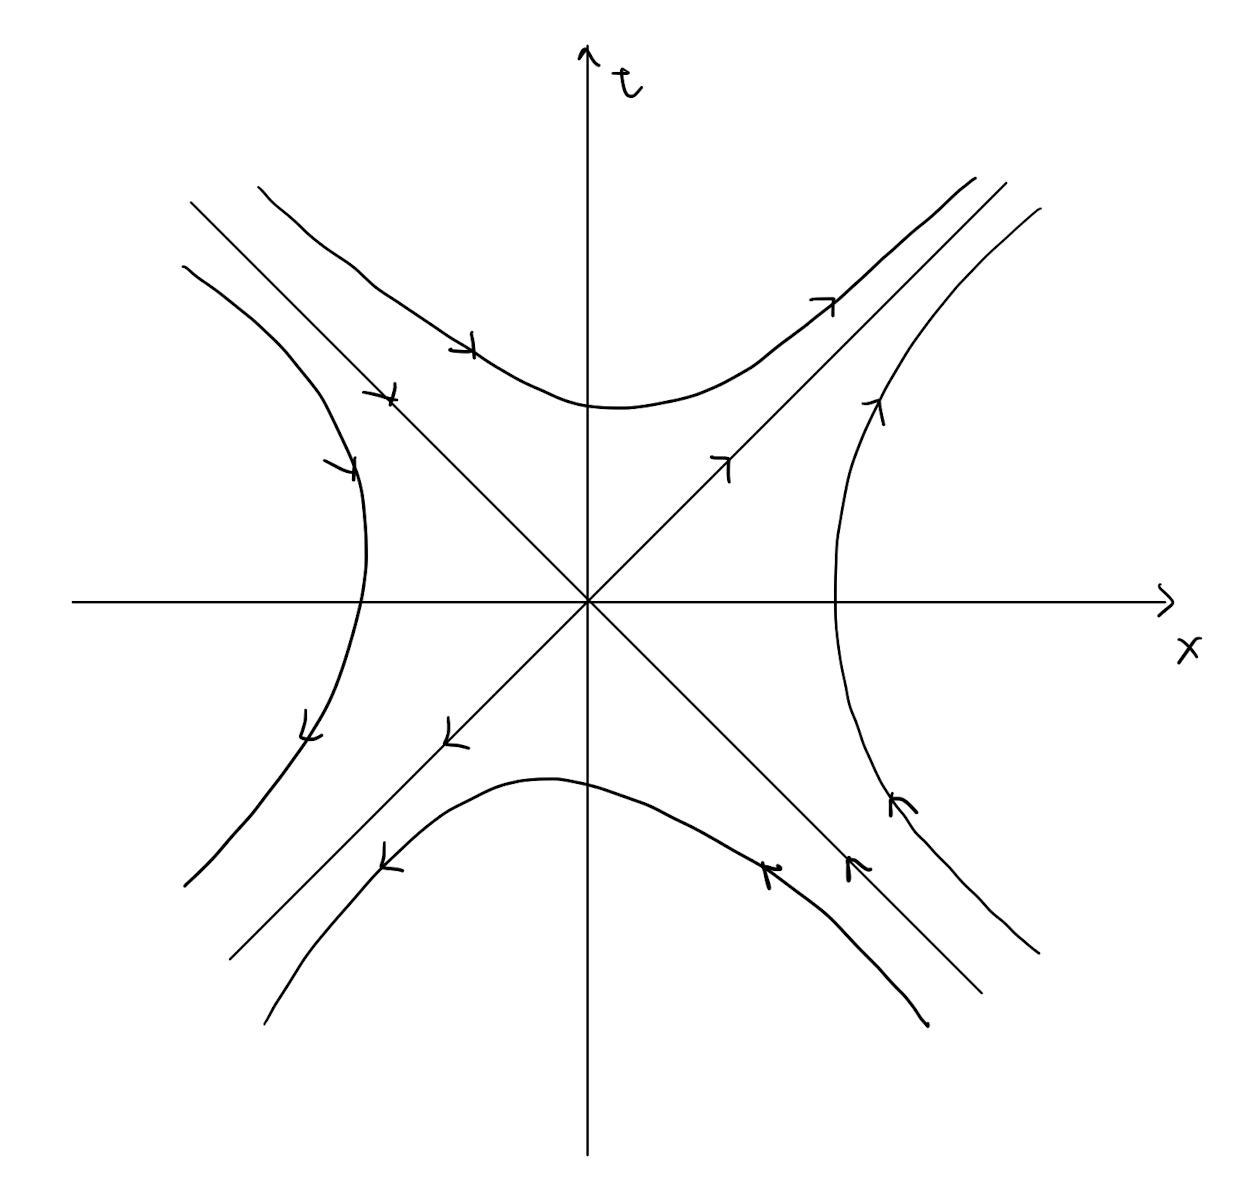
\includegraphics[width=0.5\textwidth]{pics/20-2.png}
\end{figure}
Here, we dilate the $t=x$ direction and shrink the $t=-x$ direction. This suggests that we make a change of variables $u=t+x$ and $v=-x .$ Then $\partial_{t}^{2}-\partial_{x}^{2}=4 \partial_{u} \partial_{v}$. Then the transformation $u \mapsto \lambda u, v \mapsto \lambda^{-1} v$ preserves the operator in this null frame.
\end{itemize}

\begin{theorem}
    The Lorentz group is generated by rigid spatial rotations and 1-d hyperbolic rotations.
\end{theorem}

\begin{remark}
    Hyperbolic rotations are sometimes referred to as Lorentz boosts. These hyperbolic rotations are what happens in special relativity when you switch between observers in different reference frames.
\end{remark}

We say that the solution to the wave equation is \textbf{Lorentz invariant}.

\subsection{Calculation of fundamental solutions}
We now know that the fundamental solution of the wave equation should be a "function" of $t^{2}-x^{2} .$ Here is what the picture should look like in higher dimensions.

\begin{figure}[H]
    \centering
    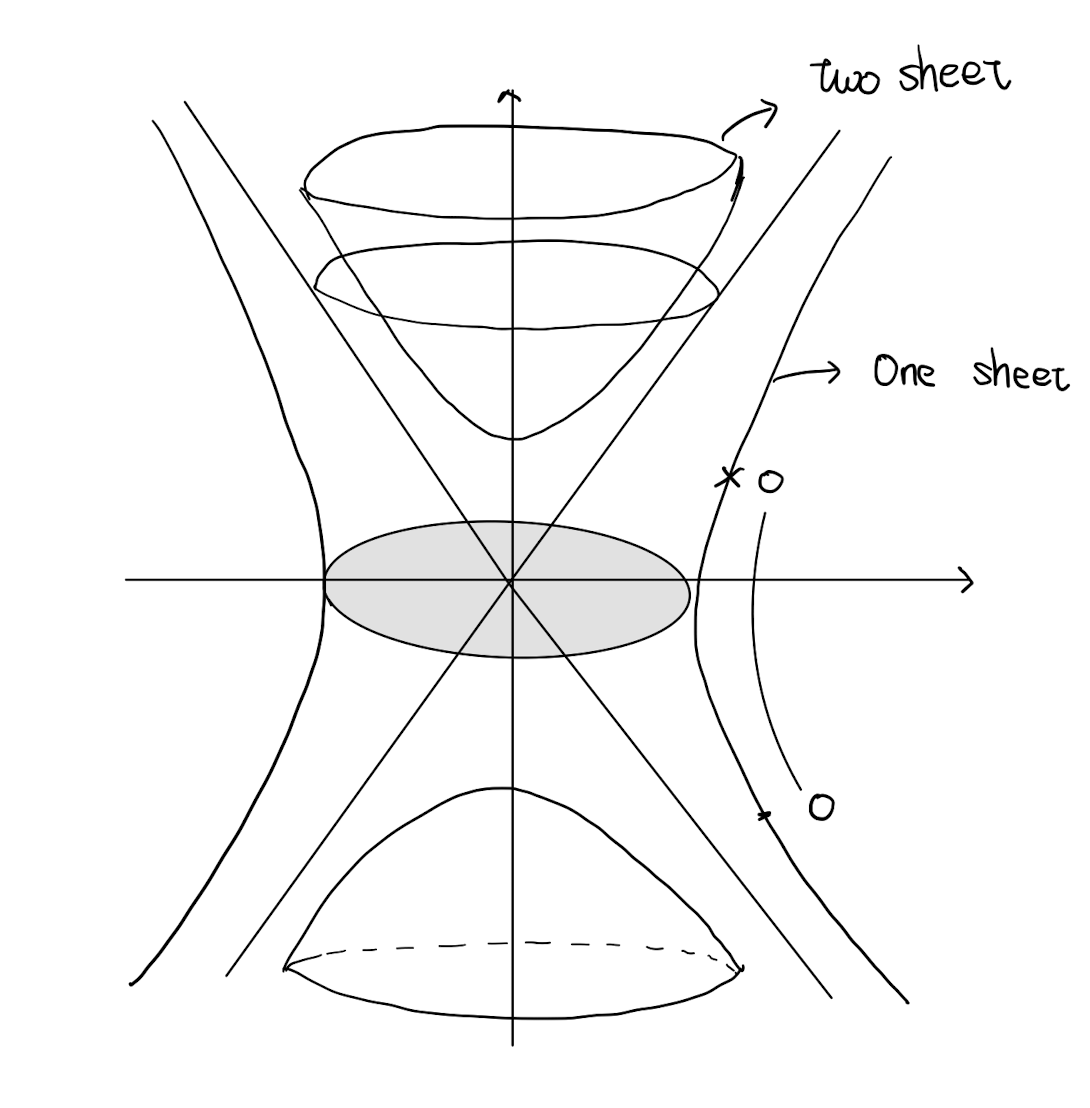
\includegraphics[width=0.5\textwidth]{pics/20-3.png}
\end{figure}

The level sets should be forward and backward cones and hyperboloids. We get 1-sheeted and 2-sheeted hyperboloids. On the 1-sheeted hyperboloids, the forward in time points are connected to the backwards in time points, which must give 0 for our forward time solution. So these must be 0 . Thus, $K=K\left(t^{2}-x^{2}\right)=K(y)$ must be supported in the forward cone $\left\{t^{2}-x^{2} \geq 0\right\}$ We want a homogeneous distribution of $y$ which is $\frac{1-n}{2}$ homogeneous (since we are now working with the squares of $t, x$ ) and supported in $y \geq 0$.

\begin{itemize}
    \item In 1 dimension, we want a homogeneous distribution of order 0 , supported where $y>0$. So $K(y)=c H(y)$, and we saw earlier that this constant is $c=1 / 2$.
    \item In 2-dimensions, we want a homogeneous distribution of order $-1 / 2$, supported where $y>0 .$ So we get
    $$
    K(y)= \begin{cases}c_{2} \frac{1}{\sqrt{y}} & y>0 \\ 0 & y \leq 0\end{cases}
    $$
    So we get
    $$
    K(t, x)=c_{2} \frac{1}{\sqrt{\left(t^{2}-x^{2}\right)_{+}}} 1_{t \geq 0}
    $$
    \item In 3 -dimensions, we cannot get a function which is homogeneous of order $-1$. The two distributions that span the space of homogeneous distributions of order $-1$ are $\delta_{0}$ and PV $\frac{1}{y}$. The latter is supported everywhere, so we take $K(y)=\delta_{y=0}$
    $$
    K(t, x)=c_{3} \delta_{t^{2}-x^{2}=0} 1_{t \geq 0}
    $$
    \item In 4 dimensions, we need homogeneity of order $-3 / 2$. However, $\frac{1}{y_{+}^{3 / 2}} \notin L_{\text {loc }}^{1}$. Define
    $$
    \frac{1}{y_{+}^{3 / 2}}:=-2 \partial_{y} \frac{1}{y_{+}^{1 / 2}}
    $$
    This is a distribution, not a function. We can repeat this differentiation procedure to get a solution for all even dimensions.
    \item In 5 dimensions, we can get a solution which is homogeneous of order -2 by differentiating $\delta_{y=0}$. We can keep differentiating to get solutions in all odd dimensions.
\end{itemize}


\subsection{Determination of constants for fundamental solutions}
Here is a formal computation: If $\square u=f$, let's see how $\int u d x$ behaves as a function of time.
$$
\begin{gathered}
\frac{d}{d t} \int u d x=\int u_{t} d x \\
\frac{d^{2}}{d t^{2}} \int u d x=\int u_{t t} d x=\int \Delta_x u+f d x=\int f d x,
\end{gathered}
$$
since we can get rid of the Laplacian using integration by parts. If $f=\delta_{0}$ and $u=K$, then $u=0$ for $t<0$, so
$$
I(t)=\int u d x=0 \quad \text { for all } t<0.
$$
Additionally, we get
$$
I^{\prime \prime}(t)=\delta_{t=0}.
$$
This tells us that
$$
I(t)=t 1_{t \geq 0}.
$$
so
$$
\int K(t, x) d x=t.
$$

\begin{itemize}
    \item In 2 dimensions, we have
    $$
    K(t, x)=\frac{c_{2}}{\sqrt{\left(t^{2}-x^{2}\right)_{+}}}
    $$
    so the equation
    $$
    t=c_{2} \int \frac{1}{\sqrt{\left(t^{2}-x^{2}\right)_{+}}} d x
    $$
    holds for all $t$. if we set $t=1$, then we get
    $$
    1=c_{2} \int_{B(0,1)} \frac{1}{\sqrt{1-r^{2}}} r d r d \theta=c_{2} 2 \pi\left[-\sqrt{1-r^{2}}\right]_{0}^{1}
    $$
    which tells us that
    $$
    c_{2}=\frac{1}{2 \pi} .
    $$

    \item In 3 dimensions, we want to find $c_{3}$. What is $\delta_{t^{2}-x^{2}} ?$
    $$
    \delta_{0}=\frac{1}{2 \pi i}\left(\frac{1}{y-i 0}-\frac{1}{y+i 0}\right)
    $$
    so we can write
    $$
    \delta_{t^{2}-x^{2}}=\frac{1}{2 \pi i}\left(\frac{1}{t^{2}-x^{2}+i 0}-\frac{1}{t^{2}-x^{2}-i 0}\right)
    $$
    Note that
    $$
    \frac{1}{t^{2}-x^{2}}= \frac{1}{t-|x|} \frac{1}{t+|x|},
    $$
    where the left term vanishes on the cone, and $t+|x|$ is $2 t$ on the cone. so we can write
    $$
    \delta_{t^{2}-x^{2}=0}=\underbrace{\delta_{t=|x|}}_{\text {surface measure on }|x|=t} \cdot \frac{1}{2 t}
    $$
    If we have a surface $\Sigma=\{\phi=0\}$, this is like normalizing to make $|\nabla \phi|=1$
    The computation becomes
    $$
    \begin{gathered}
    K(t, x)=c_{3} \frac{1}{t} \delta_{|x|=t} \\
    t=\int \frac{c_{3}}{t} \delta_{|x|=t} d x=\frac{c_{3}}{t} \underbrace{\operatorname{Area}(\{|x|=t\})}_{=4 \pi t^{2}} .
    \end{gathered}
    $$
    so we get
    $$
    c_{3}=\frac{1}{4 \pi}
    $$
\end{itemize}

\subsection{Physical interpretation of solutions to the wave equation}

Here are two key properties of the wave equation: 
\begin{itemize}
    \item [1.] All forward solutions are supported on the forward cone. This is referred as the finite speed of propagation. This says that waves move with speed $\leq 1$. If we normalize the equation with physical constants to get $c^{2} \partial_{t}^{2}-\Delta_{x}$, where $c$ is the speed of light, then this says that no waves move faster than the speed of light. An observer at position $x$ only observes the wave at the time at which the cone hits the observer's timeline:
    \begin{figure}[H]
        \centering
        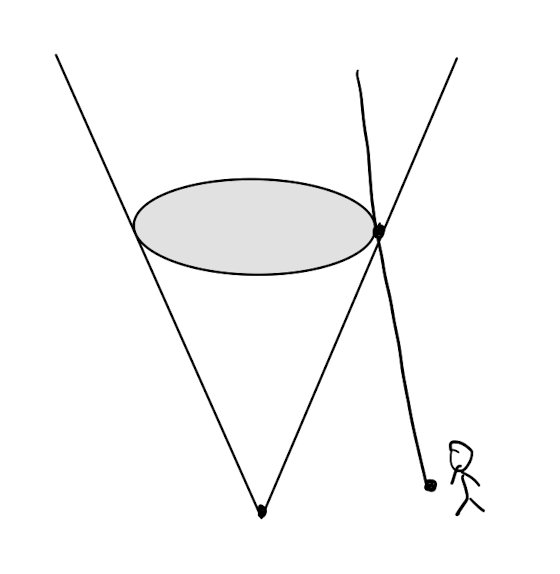
\includegraphics[width=0.4\textwidth]{pics/20-4.png}
    \end{figure}
    \item Consider 3 dimensions, where the fundamental solution $K$ is supported exactly on the cone. Here, waves hit the observer just once, and we don't see them again. This is called the Huygens principle.
\end{itemize}

\begin{remark}
    The equations of physics are nonlinear; this linear PDE is just the best linear approximation. The finite speed of propagation remains, but Huygen’s principle does not hold in general. When scientists observed gravitational waves recently, they observed both a Dirac mass and a nonlinear tail.

    \begin{figure}[H]
        \centering
        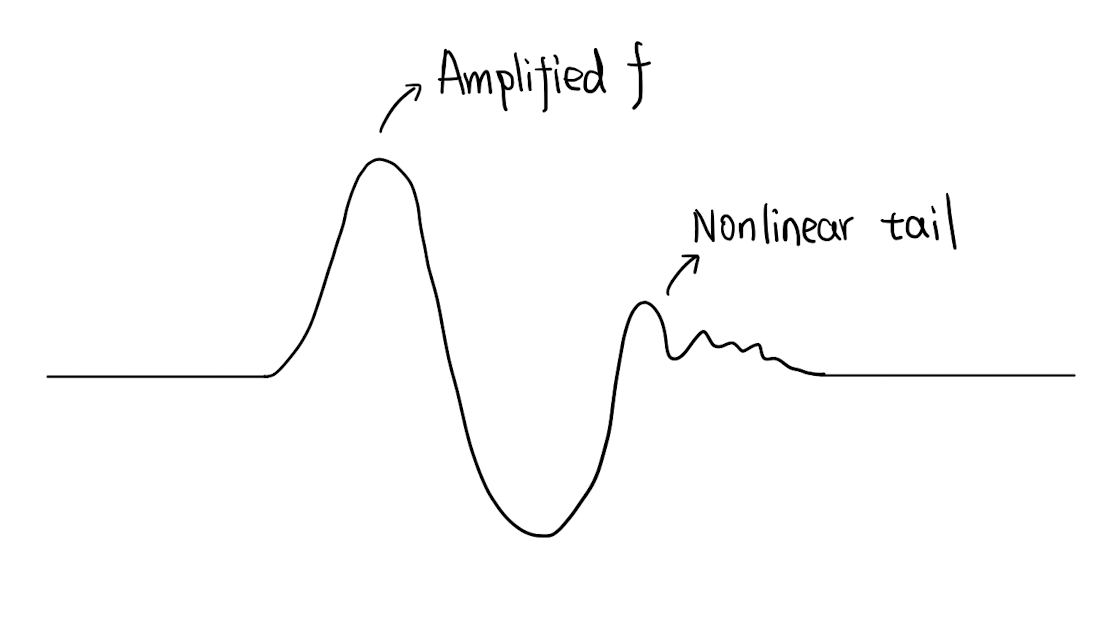
\includegraphics[width=0.4\textwidth]{pics/20-5.png}
    \end{figure}
\end{remark}

\subsection{Next steps: Fourier series}
Our next goal is to learn about the connection between the Fourier transform and Fourier series. The Fourier transform $\widehat{u}$ of $u: \mathbb{R}^{n} \rightarrow \mathbb{C}$ is given by
$$
u(x)=\int \widehat{u}(\xi) e^{i x \cdot \xi} d \xi
$$
\text { In calculus, you may have encountered Fourier series: }

\begin{definition}
    [Fourier series]
    If $u:[0,2 \pi] \rightarrow \mathbb{C}$, then the Fourier series for $u$ is given by $u(x)=\sum_{n} c_{n} e^{i n x}=\sum_{n} c_{n}(\cos (n x)+i \sin (n x))$
\end{definition}
Not all PDEs can be solved; we will see more about this next time.